% Please do not change the document class
\documentclass{scrartcl}

% Please do not change these packages
\usepackage[hidelinks]{hyperref}
\usepackage[none]{hyphenat}
\usepackage{setspace}
\usepackage{graphicx}
\doublespace

% You may add additional packages here
\usepackage{amsmath}

% Please include a clear, concise, and descriptive title
\title{How the use of Personas in Agile may Allow Game Developers to Construct more Focused and Prioritised User Stories}

% Please do not change the subtitle
\subtitle{COMP150 - Agile Essay}

% Please put your student number in the author field
\author{1507290}

\begin{document}

\maketitle

\abstract{Agile agile agile abstract}

\section{Introduction}
The Agile methodology itself does not directly address usability. The Agile Manifesto~\cite{manifesto} is focused on the development process from the team's perspective. Although the Agile Manifesto refers to ``customer collaboration'', this is likely referring to the product owner, rather than the consumers of the product. Despite some conflicts in principles, interest in incoorporating user-centred design (UCD) methods into Agile is growing~\cite{haikara:extending}. One such UCD tool which has been integrated into some Agile methods is the use of personas~\cite{caballero:persona}. Personas are a set of fictional characters created to be archetypal of the different groups of intended users. Their primary purpose is to solidify the concept of the end user to help designers and developers more effectively understand the product's intended users~\cite{}. 
Games are solely about the player's experience of the game, so an understanding of the user is especially important. This essay will explore how the use of personas in an agile games development process could help create a game that provides the player with a better experience, as well as helping the team construct and prioritise user stories more effectively.

\section{The Benefits of Using Personas}
Personas can help designers, developers and testers more effectively capture the needs of their intended product users, as well as being a tool to aid communication~\cite{}. Personas usually contain information about the user such as name, age, occupation, a photo, and the goals of that Persona when using the product. In agile, they are usually placed on the task board or in a notable place in the team's working environment \cite{}. The use of personas can help developers and designers more carefully consider how users would use the product and what their goals are, since they are concretely defined rather than abstract sections of the target market. Furthermore, designing a product for personas is likely to result in a product that caters to the needs of the intended users, as not only do they solidify the concept of the user, but also are based on research and empiracle data collected about the intended users~\cite{}. This also means that the team has a shared understanding of who they are designing for, instead of working from personal assumptions. This is made more effective as personas should be based on research into the potential users. Understanding how the user will experience the product is especially important in a field such as games, which must provide the player with an enjoyable and engaging experience.

\section{Integrating Personas into Agile}
Some elements of Personas conflict with elements of the Agile manifesto, whilst some parts of their philosophies are similar~\cite{haikara:extending, chaimberlain:framework}. The Persona method in UCD usually involves researching the users and creating the personas before any development begins, whereas Agile discourages this practice~\cite{chaimberlain:framework}. In order to make personas compatible with Agile, they could be made to be iterative, as is demonstrated with `Extreme Personas'~\cite{wolkerstorfer:probing}. This way, the persona's profile would be reviewed and developed alongside the project as requirements change and new information about the potential players surface. The personas could be reviewed at the end of each sprint, alongside user stories. Furthermore, personas could inform the priorty of user stories, by using their goals and personalities as a guide~\cite{microsoft thing}: stories that positively affect the most personas could be prioritised more highly.
This could ensure that the team is making more effective use of it's time by working on user stories that are going to affect the players the most.

%Developing personas alongside user stories may help the user stories be more user based and informed.

\section{How can Personas be Used in Game Development?}
It is difficult to focus user stories on users in game development; all of the users are 'players'. Using personas could provide a way to target the user stories at specific types of player. 
Another approach to tying personas to user stories is to create persona driven user stories~\cite{winter:vision}; that is, user stories that specifically refer to a single persona. Perhaps this could be extended by adding versions of the user story from the point of view of each individual persona to the main user story. This way, it will make it clear how a given feature will affect different types of players' experiences of the game. The goals of the persona will be of particular importance; they define the player's motivations for playing the game and what they want to achieve. 
\begin{figure}[h]
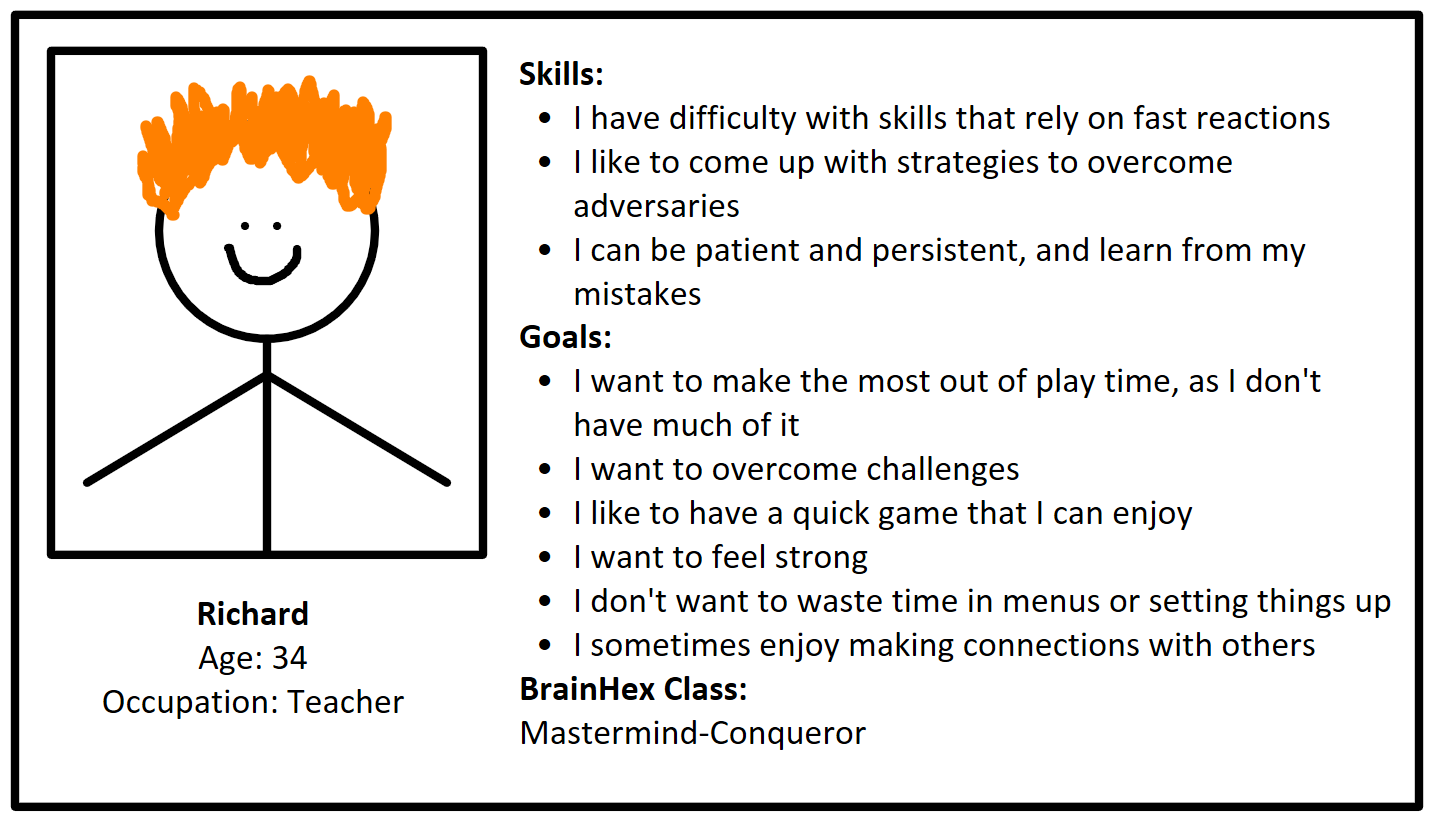
\includegraphics[width=\textwidth]{example.png}
\caption{An example of a Persona for game development}
\label{fig:persona_example}
\end{figure} 
In addition to specifying particular goals, the persona's motivations and characteristics could be supplemented by the inclusion of information about the player's gamer type according to taxonomies such as Brainhex~\cite{nacke:brainhex}, the Bartle test\cite{bartle:mud}, or Yee's taxonomy\cite{yee:online}. To make the most effective use of this information, the team members will need to become familiar with the taxonomy used. For the general case, Brainhex is likely to be the most useful for giving a general overview of the player's characteristics, as the other two are targeted at player behaviour in online games. An example of the information a game development persona could include is illustrated in Figure~\ref{fig:persona_example}. 

\section{Conclusion}
With certain alterations and additions, personas could be an effective tool to use in an agile games development process, at the expense of additional time spent researching the users and constructing the personas. They have the potential to allow the team to better prioritise their user stories, resulting in a more effective use of development time. Providing they are based on empirical data about the potential players, the use of personas will ensure that the team has a shared perception of who they are producing the game for. Understanding between difference departments may also be enhanced by using the personas as a communication tool for raising and addressing issues.

\bibliographystyle{ieeetran}
\bibliography{comp150_agile}

\end{document}
